\documentclass[../TST.tex]{subfiles}
\begin{document}
\begin{pproblem}
	A particle of mass $m$ and charge $q$ moves under a constant magnetic field $B$ and an alternating electric field $E(t)=E_m\cos{(\omega t)}$, where $\omega = \frac{qB}{m}$. At time $t=0$ the particle is at rest at the centre of the coordinate system (Figure 1). Find the classical equations of motion of the particle $x(t)$, $y(t)$, and $z(t)$. Describe the shape of the trajectory. \\[5pt]
\textit{Hint:} The motion along $Oy$ is described by a function of the form $y(t)=At\sin{(\omega t)}$.\\
\begin{figure}[H]
\centering
    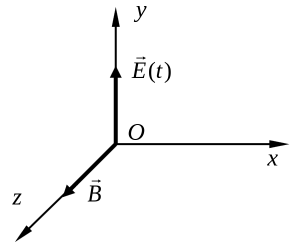
\includegraphics[width=0.4\textwidth]{fig/2012_s3.png}
  \caption{}
  \label{fig1}
  \end{figure}

\end{pproblem}

\ifprob \else
	\begin{solution} This problem is nearly identical to Problem 5 from 2011, though a bit heavier on the calculations. To start with, we will note that the total force $\mathbf{F}=q\mathbf{v}\times \mathbf{B}+q\mathbf{E}$ is constrained to the $xy$-plane, and because the particle is initially at rest, it will always remain in that plane. Thus, \fbox{$z(t)=0.$}\\[5pt]
The components of the force in the $xy$-plane are
	\begin{align*}
		F_x &= m \frac{\mathrm{d}v_x}{\mathrm{d}t}=qv_yB,\\
		F_y &= m \frac{\mathrm{d}v_y}{\mathrm{d}t}=qE_m\cos{(\omega t)}-qv_xB.
	\end{align*}
The hint tells us something about $y(t)$, so we would like to obtain an equation in $v_y$ only. We differentiate the second equation and then refer to the first one to reach
\begin{equation*}
	\frac{\mathrm{d}^2v_y}{\mathrm{d}{t}^2}+\omega^2v_y=-\omega^2 \left(\frac{E_m}{B}\right)\sin{(\omega t)}
.
\end{equation*}
Let us work with $y(t)=A_1(\omega t)\sin{(\omega t)}$, where $A_1\omega=A$. It's a bit easier to take derivatives with respect to $(\omega t)$ rather than $t$. Using $\frac{\mathrm{d}}{\mathrm{d}t}=\omega \frac{\mathrm{d}}{\mathrm{d}(\omega t)}$, we get
\begin{align*}
	v_y&=A_1\omega (\sin{(\omega t)}+(\omega t)\cos{(\omega t)})
,\\
	\dot{v}_y&=A_1\omega^2 (2\cos{(\omega t)}-(\omega t)\sin{(\omega t)})
,\\
	\ddot{v}_y&=A_1\omega^3 (-3\sin{(\omega t)}-(\omega t)\cos{(\omega t)})
.
\end{align*}
Matching both sides of the differential equation, we see that
\begin{equation*}
	-2A_1\omega^3\sin{(\omega t)}=-\omega^2 \left(\frac{E_m}{B}\right) \sin{(\omega t)},
\end{equation*}
or $A=A_1\omega = \frac{E_m}{2B}$. As a result, $\boxed{y(t)=\frac{E_m}{2\omega B}(\omega t)\sin{(\omega t)}.}$\\[5pt]
Now we turn to $x(t)$. Having found $A$, we can get $v_x$ from the $F_y$ equation:
\begin{equation*}
	v_x=\frac{E_m}{B}\cos{(\omega t)}- \frac{1}{\omega}\frac{\mathrm{d}v_y}{\mathrm{d}t}=\frac{E_m}{2B}(\omega t)\sin{(\omega t)}
.
\end{equation*}
Finally, integrating this with $x(0)=0$ gives us
\begin{equation*}
	\boxed{x(t)=\frac{E_m}{2\omega B}\left(-(\omega t)\cos{(\omega t)}+\sin{(\omega t)}\right).}
\end{equation*}
You should double-check that the initial conditions $x(0)=0$, $y(0)=0$, $v_x(0)=0$, and $v_y(0)=0$ are all satisfied. You could also replace $\omega$ with $\frac{qB}{m}$ in the final answers if you feel like it. \\[5pt]
The trajectory is a \fbox{spiral}, as shown. In the equation for $x(t)$ there is a harmonic term $\sim \sin{(\omega t)}$ which becomes negligible as $\omega t \rightarrow \infty$, when the other terms will blow up. Those terms correspond to an Archimedean spiral $r(\varphi)=A\varphi$. It is fair to say that our trajectory asymptotes to an Archimedean spiral.
\begin{center}
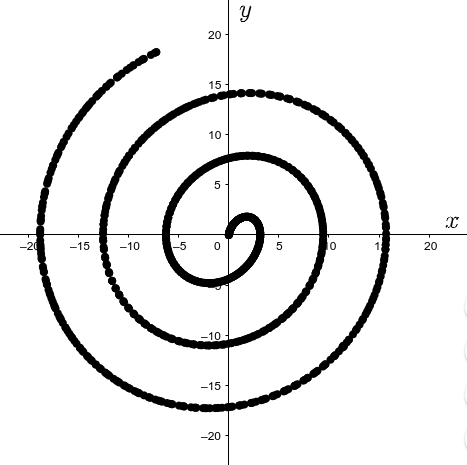
\includegraphics[width=0.5\textwidth]{fig/a2012_s3.png}
\end{center}

\end{solution}
\fi
\end{document}
